% Fig. 2 -- Button event recognizer M_B (timed Mealy machine).
% Source: firmware/esp32c3_oled_mqtt/esp32c3_oled_mqtt.ino, function readButton().
\documentclass[border=4pt]{standalone}
\usepackage{mathptmx}
\usepackage{amsmath}
\usepackage{tikz}
\usetikzlibrary{automata,positioning,arrows.meta,calc}
\begin{document}
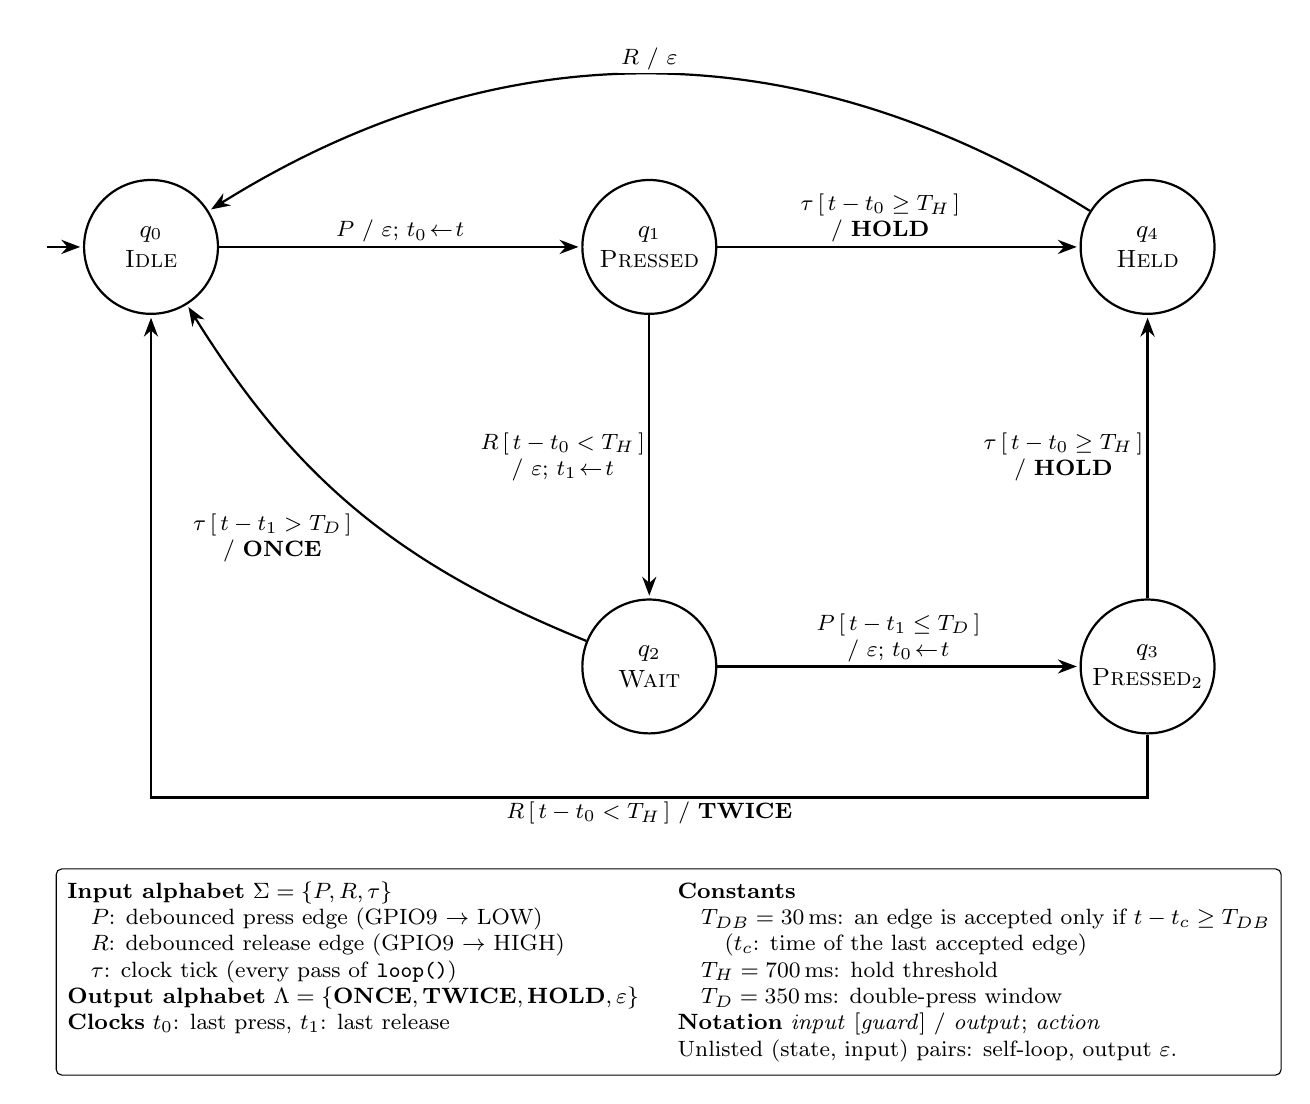
\begin{tikzpicture}[
    >={Stealth[length=2.4mm]},
    shorten >=1pt, node distance=4.6cm, auto,
    every state/.style={draw, thick, minimum size=17mm, align=center, inner sep=1pt, font=\small},
    lab/.style={font=\footnotesize, align=center, fill=white, inner sep=1.2pt},
    every edge/.style={draw, thick}]

  % states
  \node[state, initial, initial text={}] (q0) {$q_0$\\ \textsc{Idle}};
  \node[state, right=of q0]                (q1) {$q_1$\\ \textsc{Pressed}};
  \node[state, right=of q1]                (q4) {$q_4$\\ \textsc{Held}};
  \node[state, below=3.6cm of q1]          (q2) {$q_2$\\ \textsc{Wait}};
  \node[state, below=3.6cm of q4]          (q3) {$q_3$\\ \textsc{Pressed}$_2$};

  % transitions:  input [guard] / output ; action
  \path[->]
    (q0) edge node[lab] {$P$ / $\varepsilon$;\ $t_0\!\leftarrow\!t$} (q1)
    (q1) edge node[lab, pos=.45] {$\tau\,[\,t-t_0 \ge T_H\,]$\\ / \textbf{HOLD}} (q4)
    (q1) edge node[lab, left, pos=.5] {$R\,[\,t-t_0 < T_H\,]$\\ / $\varepsilon$;\ $t_1\!\leftarrow\!t$} (q2)
    (q2) edge node[lab] {$P\,[\,t-t_1 \le T_D\,]$\\ / $\varepsilon$;\ $t_0\!\leftarrow\!t$} (q3)
    (q3) edge node[lab, left] {$\tau\,[\,t-t_0 \ge T_H\,]$\\ / \textbf{HOLD}} (q4)
    (q2) edge[bend left=18] node[lab, pos=.5] {$\tau\,[\,t-t_1 > T_D\,]$\\ / \textbf{ONCE}} (q0)
    (q4) edge[bend right=32] node[lab, above] {$R$ / $\varepsilon$} (q0)
    ;
  \draw[->, thick] (q3.south) -- ++(0,-0.8) -| node[lab, pos=.25, below] {$R\,[\,t-t_0 < T_H\,]$ / \textbf{TWICE}} (q0.south);

  % legend
  \node[draw, rounded corners=2pt, align=left, font=\footnotesize, anchor=north west, inner sep=4pt]
    at ($(q0.south west |- q3.south)+(-0.6,-1.7)$) {%
    \begin{tabular}{@{}l@{\hspace{14pt}}l@{}}
    \textbf{Input alphabet} $\Sigma=\{P, R, \tau\}$ & \textbf{Constants}\\
    \quad $P$: debounced press edge (GPIO9 $\to$ LOW) & \quad $T_{DB}=30$\,ms: an edge is accepted only if $t-t_c \ge T_{DB}$\\
    \quad $R$: debounced release edge (GPIO9 $\to$ HIGH) & \quad\quad ($t_c$: time of the last accepted edge)\\
    \quad $\tau$: clock tick (every pass of \texttt{loop()}) & \quad $T_H=700$\,ms: hold threshold\\
    \textbf{Output alphabet} $\Lambda=\{\textbf{ONCE},\textbf{TWICE},\textbf{HOLD},\varepsilon\}$ & \quad $T_D=350$\,ms: double-press window\\
    \textbf{Clocks} $t_0$: last press,\ $t_1$: last release & \textbf{Notation} \textit{input} [\textit{guard}] / \textit{output}; \textit{action}\\
    & Unlisted (state, input) pairs: self-loop, output $\varepsilon$.
    \end{tabular}};
\end{tikzpicture}
\end{document}
